\documentclass{article}

\usepackage{arxiv}

\usepackage{hyperref}       % hyperlinks (but not footnotes: bug points links to titlepage)
\usepackage{url}            % simple URL typesetting
\usepackage{booktabs}       % professional-quality tables
\usepackage{amsfonts}       % blackboard math symbols
\usepackage[T1]{fontenc}	% font encoding
\usepackage{palatino}		% font typefaces
\usepackage{nicefrac}       % compact symbols for 1/2, etc.
\usepackage{microtype}      % microtypography
\usepackage{setspace}		% line spacing
\usepackage{lipsum}
\usepackage{graphicx}
\usepackage{tabularx}
\usepackage{pdflscape}
\usepackage{doi}
\renewcommand{\doitext}{}	% avoid "doi: doi:" in references lists

\usepackage{xcolor}

% References format
\usepackage[natbibapa]{apacite} % APA 6th ed. styling for citations and references list
\bibliographystyle{apacite}


\graphicspath{{figures/}}

%%
%% Circled numbers
%%
\usepackage{tikz}
\newcommand*\circled[1]{\tikz[baseline=(char.base)]{
	\scriptsize\node[shape=circle,draw,inner sep=1pt] (char) {#1};}}

%%
%% Line spacing
%%
\setstretch{1.32} 

\title{Exploring the Role of Adaptive Hybrid Intelligent Systems on Competitive Advantage Using a Case From the STM Publishing Industry}

\author{Dietrich Rordorf\\
	\href{mailto:dietrichhanspaul.rordorf@students.fhnw.ch}{dietrichhanspaul.rordorf@students.fhnw.ch} \\
	\AND
	Supervisor: Dr. Emanuele Laurenzi \\
	\\
	School of Business \\
	University of Applied Sciences and Arts Northwestern Switzerland \\
	Riggenbachstrasse 16 \\
	CH-4600 Olten \\
	Switzerland \\
}
\date{
	MSc Business Information Systems Program \\
	Emerging Topics, SS 2023
}

% Uncomment to remove the date
%\date{}

% Uncomment to override  the `A preprint' in the header
\renewcommand{\headeright}{Draft}
\renewcommand{\undertitle}{Semester Paper}
\renewcommand{\shorttitle}{Competitive Advantage of Hybrid Intelligent Systems}

%%% Links within PDF and PDF metadata
\hypersetup{
	unicode=true,
	bookmarksopen={true},
	pdffitwindow=true,
	colorlinks=true,
	allcolors=black,
	hidelinks=false,
	hyperfootnotes=false,
	pdfstartview={FitH},
	pdfpagemode=UseNone,
	pdftitle={Enhancing Enterprise Competitiveness through Adaptive AI Systems},
	pdfauthor={Dietrich Rordorf},
	pdfkeywords={artificial intelligence, hybrid intelligence, adaptive AI systems, enterprise competitiveness},
}

\begin{document}

%%% Title page
\maketitle
\begin{abstract}
    {\color{purple} @todo: write the abstract once the paper is ready\dots}
\end{abstract}

%%% Table of contents
\newpage
\tableofcontents
\newpage

%%% Content sections
\section{Introduction}
\label{sec:introduction}

As enterprises face universally accelerating change \citep{eliazarUniversalityAcceleratingChange2018}, it
is crucial for their artificial intelligence (AI) systems to be dynamic and adaptable. Hybrid intelligent (HI)
systems that learn from both new data and the interaction with human agents can provide a competitive advantage
to enterprises. This study explored the competitive advantage for enterprises adopting adaptive hybrid intelligent
systems using the case of a typical editorial process in the scientific, medical and technical (STM) publishing
industry. The study answers the following research question: \textit{How can AI systems learn from and adapt
to humans and their environment for the competitive advantage of enterprises?}

A mixed-methods approach was used, consisting of a literature review and qualitative data collection from
a focus group of graduate students in information systems ($n = 25$). The literature review identified how 
adaptive hybrid intelligent systems contribute to competitive advantages and was used to derive hypotheses
using the case of the scientific, medical and technical (STM) publishing industry. The hypotheses were
tested through qualitative feedback from the focus group.

{\color{purple} @todo: after the workshop, add a short summary of the main hypotheses, findings, 
discussions and conclusion\dots}

The remainder of the paper is structured as follows. Section \ref{sec:literature} presents a literature review
on hybrid intelligent systems and their competitive advantage for enterprises. Section \ref{sec:methods} describes
the methodological approach of the study. Section \ref{sec:results} presents the findings. The paper concludes in
Section \ref{sec:discussion} with a discussion of the findings and limitations of the study.
\section{Literature Review}
\label{sec:literature}

In this section we inform a background on different types of artificial intelligence (AI), hybrid intelligence, 
design patterns and principles for hybrid intelligent systems, and the competitive advantage arising from
the use of such systems in enterprises.

\subsection{Categorization of AI}

According to \cite{russel2010} AI is the creation of computer programs and algorithms that allow machines to
replicate human cognition and behavior, which includes the capabilities of learning, perception, reasoning,
solving problems, and making decisions. AI can be broadly subdivided into symbolic and sub-symbolic approaches,
see e.g., \cite{eliasmithSymbolicSubsymbolic2006}. Symbolic approaches involve the use of explicit symbols and
rules to represent knowledge and reason in a way that is easily understood and explainable by humans, while sub-symbolic
(or \textit{connectionist}) approaches aim to learn complex patterns from vast amounts of data using neural
networks \citep{ilkouSymbolicVsSubsymbolic2020}.

Hybrid AI refers to systems involving symbolic and sub-symbolic approaches. Hybrid AI systems can be anywhere from
loosely coupled to tightly integrated \citep{garcezNeurosymbolicAI3rd2020}. Loosely coupled hybrid AI systems typically
involve a human, which is also known as \textit{human in the loop} (HITL) computing. In such systems the humans and
AI work together towards common goals, augmenting the human intellect and overcoming human limitations and cognitive
biases \citep{akataResearchAgendaHybrid2020}. The hybrid systems show the  potential for improving the outcomes of AI
systems, hence \textit{augmenting} rather than replacing human intelligence \citep{akataResearchAgendaHybrid2020}.
Within tightly integrated hybrid AI approaches, neurosymbolic AI has earned a particular research interest as a possible
way to overcome the limitations of deep learning, such as lack of explainability, susceptibility to adversarial attacks
(data poisoning) and high computational cost \citep{garcezNeurosymbolicAI3rd2020}. Hybrid intelligence has recently
received attention from the leaders in the field: in his presidential address to the AAAI community, 
\cite{kambhampatiChallengesHumanAwareAI2020} demanded that AI researchers build human-aware AI systems that consider
the human mental model. In particular, AI researchers should aim at systems that show the capabilities of \textit{explicability}
(AI agents should show behavior that is expected by humans) and \textit{explainability} (AI agents -- if behaving unexpectedly -- 
should be able to provide an explanation) \citep{kambhampatiChallengesHumanAwareAI2020}.

Another way to categorize AI is by the breadth of application. The 
- Narrow AI

- Neuro-symbolic AI as a promising way to reach broad AI \citep{@hochreiterBroadAI2022}.

- General AI, also Artificial General Intelligence (AGI)


Hybrid AI architectures:

- Agents

- 


\subsection{Design Principles for Hybrid Intelligent Systems}

Hybrid AI systems can be represented by a boxology notation with common design patterns \citep{harmelenBoxologyDesignPatterns2019,
vanbekkumModularDesignPatterns2021,witschelVisualizationPatternsHybrid2021}.

\cite{ostheimerAllianceHumansMachines2021} developed a framework of eight principles for the design of human-in-the-loop (HITL) 
computing. They argue that such hybrid systems achieve higher accuracy and reliability of machine learning algorithms. Using a 
case in the manufacturing industry, they showed that the efficiency of operational processes could be increased by applying an 
algorithm that followed these design principles \citep{ostheimerAllianceHumansMachines2021}.

% box with HITL design principles
{
    \begin{center}
        \vskip 0.2in
        \fcolorbox{gray}{white}{
        \parbox{0.85\textwidth}{
        \textbf{Box 1. HITL Computing Design principles \citep{ostheimerAllianceHumansMachines2021}.}
        \begin{enumerate}
            \item Principle of client-designer relationship: designers should aim for mutual knowledge exchange with clients to foster the understanding
                    of which aspects of a system are influenced by human or artificial intelligence.
            \item Principle of sustainable design: designers should keep up to date with the latest progress in the field of AI and apply the latest and
                    lasting AI techniques.
            \item Principle of extended vision
            \item Principle of AI-readiness
            \item Principle of hybrid intelligence
            \item Principle of use-case marketing
            \item Principle of power relationship
            \item Principle of human-AI trust
        \end{enumerate}}}
        \vskip 0.2in
    \end{center}
}


\subsection{Narrow versus Broad AI}

\subsection{Artificial General Intelligence (AGI)}



\subsection{Types of Hybrid Intelligent Systems}

\begin{itemize}
    \item Expert systems 
    \item Decision support systems
    \item Recommender algorithms with human decision-making
    \item Case-based reason systems
\end{itemize}


\subsection{Foundation Models}

\begin{itemize}
    \item Language Models (LMs)
    \item neural networks trained of vast amounts of data, including on multimodal data (text, images, speech, video)
    \item Good at a variety of tasks, often the performance of LMs is closed to that of specialized model
    \item However, they show several limitations in their capabilities in reasoning and information retrieval. 
    \item Thus the terms "Foundation Model" was proposed by researchers at the Human-centered AI (HAI) institute of Stanford University
\end{itemize}

\begin{itemize}
    \item Foundation models represent a paradigm shift in AI
    \item ChatGPT as a chatbot is highly interactive: user has to prompt AI (althoug it is an unexplainable black box)
    \item Emerging capability in foundation models: in-context learning 
    \item In-context learning is highly adaptable: AI can learn from examples in the prompt 
\end{itemize}

\subsubsection{Limitations of Foundation Models}

\subsubsection{Hybrid Intelligent Approaches Involving Foundation Models}

\begin{itemize}
    \item Agents 
    \item Mixed architecture, e.g., MRKL
    \item Using the model as IR agent 
\end{itemize}





\subsection{Enterprise Competitiveness}

{\color{purple} @todo: what are the aspects of and factors increasing the competitiveness of enterprises?}


\subsection{Competitive Advantage Through Adaptive Hybrid Intelligent Systems}

\cite{xuCanArtificialIntelligence2021} found that post COVID-19 companies using AI in their products grew
faster than their peers. However, they could not observe evidence of the same effect before COVID-19, indicating
that this development is either very recent or was fueled by the COVID crisis. More recently
\cite{hoArtificialIntelligenceFirm2022} reviewed the potential benefits of AI for enterprises as reported
by selected previous studies published between 2016 and 2021:

\begin{itemize}
    \item reduced costs
    \item improved performance
    \item better decision-making
    \item higher customer satisfaction
    \item better customer segmentation
    \item improved customer experience
    \item better products \& services
    \item business innovation
\end{itemize}

Further, \cite{hoArtificialIntelligenceFirm2022} identified several empirical studies that reported a positive,
neutral or negative effect of AI on enterprise performance. In particular one study by ...liu et al. (2022)...
and cited in \cite{hoArtificialIntelligenceFirm2022} reported negative performance of AI-related adoption 
announcements on firm market value for 62 listed US companies between 2015-2019.

\section{Methodology}
\label{sec:methods}

The study aimed to investigate the competitive advantage that can arise for an enterprise
through the adoption of hybrid intelligent systems. Specifically, the study explored the aspect of adaptability
of such hybrid intelligent systems. The study used a mixed-methods approach consisting of a literature
review (secondary data) and qualitative data collection from a focus group of 25 graduate students in the
FHNW Business Information Systems master program (primary data).

The literature review was conducted to identify factors that contribute to the competitive advantage
of enterprises using AI systems in general, and adaptable hybrid intelligent systems in particular.
The literature search was mainly conducted on Elicit \footnote{\href{https://elicit.org/}{elicit.org}}
and Google Scholar \footnote{\href{https://scholar.google.com/}{scholar.google.com}} using different
query terms, including ``competitive advantage of AI'', ``hybrid intelligent system'',
``expert system'', ``decision support system'', ``human-in-the-loop'', ``competitive advantage and AI'',
etc. Additionally, a forward and backward search was applied on relevant papers that were identified
from the initial literature searches.

The findings from the literature review were used to establish hypotheses on the competitive advantage
of adaptable hybrid intelligent systems for enterprises using the example of one industry. Given the
background knowledge of the author, the hypotheses were applied to the scientific, technical and medical
(STM) publishing industry. To test the derived hypotheses, a focus group of students ($n = 25$) was selected
based on their educational background in business information systems. As part of a workshop the focus group
was presented with the hypotheses and asked to discuss and provided qualitative feedback for each hypothesis.
Participants were encouraged to provide detailed feedback on their experiences and perceptions related
to the application of the hypotheses in the industry case. The qualitative data was analyzed using
thematic analysis and common themes identified.
\section{Results}
\label{sec:results}

\subsection{The Editorial Process}

A simplified, typical editorial process -- from writing to the final decision -- for a manuscript submitted to a scholarly journal is shown in
Figure ~\ref{fig:bpmnEditorialProcess}. The process includes at least three parties: the author who writes the manuscript, the editor of the
journal or conference chair that coordinates the peer-review process, and the peer-reviewers that review and comment on a manuscript. Towards
the end of the writing process, the author will start to think about the journal (or conference) where he/she wants to submit the paper to.
Once the author identified a journal, the manuscript has to be formatted to meet the submission requirements of the journal. 
{\color{purple} @todo: textual description of process steps \dots}

\begin{figure*}[htb]
    \centering
    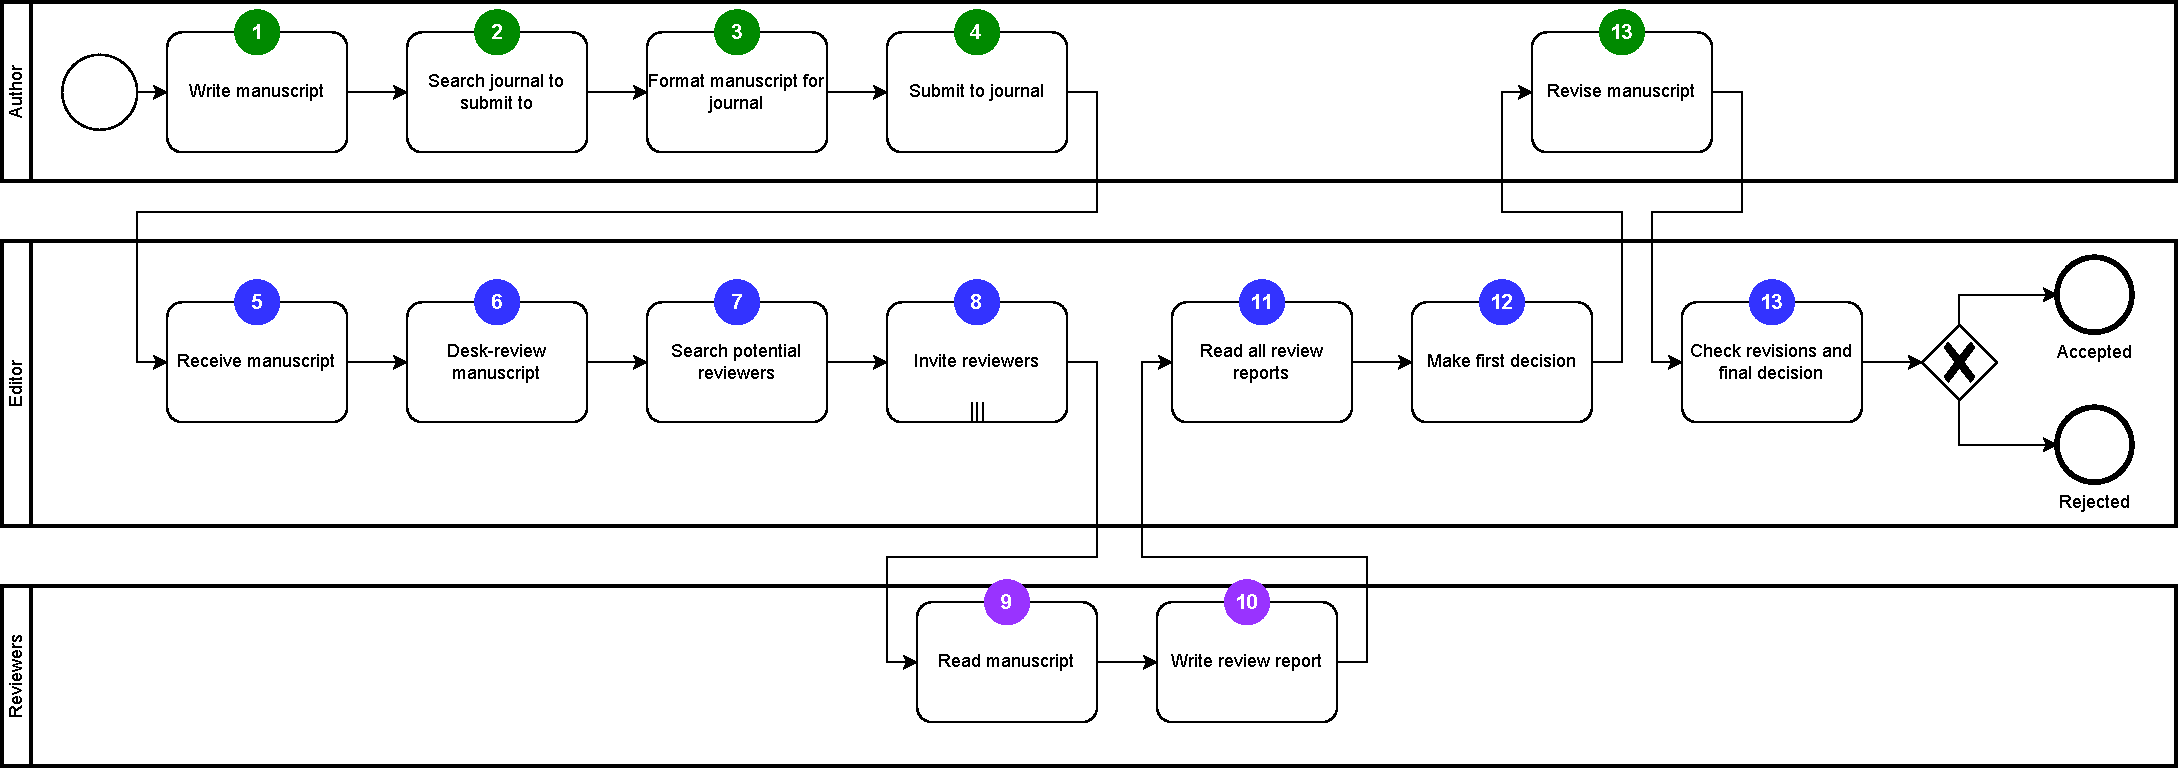
\includegraphics[width=\linewidth]{editorial_process.pdf}
    \caption{A simplified, typical editorial process from writing the manuscript to the final decision of acceptance or
    rejection for publication (in BPMN 2.0). For better understanding, the process steps performed by outside parties 
    are also modelled and the process starts with the outside party (author) writing the manuscript. The numbers
    indicate the sequence flow of the process.}
    \label{fig:bpmnEditorialProcess}
\end{figure*}

\subsection{Use Cases For AI in the Editorial Process}

Table  ~\ref{tab:editorialProcess} shows an overview of the use cases for hybrid AI systems for each step in the typical editorial process.
{\color{purple} @todo: then we can pick those areas where adaptive hybrid AI could be interesting and reason why so\dots}


\subsection{Step XY}

{\color{purple} @todo: then we can pick exactly one adaptive hybrid AI use case, draw 1-2 hypotheses that we can research 
during the workshop\dots}


\begin{landscape}
    \begin{table}[htb]
        \caption{
            Typical editorial processing steps and use cases for (hybrid) AI for a scholarly journal.
            {\color{purple} @todo: refine table \dots}
        }
        \label{tab:editorialProcess}
        \renewcommand{\arraystretch}{1.25}
        \small\centering
        \setlength\tabcolsep{6pt}
        \begin{tabularx}{\linewidth}{l l l X}
            \toprule
            \textbf{Step} & \textbf{Role} & \textbf{Task} & \textbf{Use Cases for Hybrid AI} \\
            \midrule

            \circled{1} & Author & Writes manuscript & AI-aided writing, translating, grammar and spell-checking,
                AI-aided literature search and literature review\\

            \circled{2} & Author & Searches for journals to submit to & Decision support system with AI-guided journal recommendation
                based on word embeddings of the manuscript and knowledge engineering using the academic graph\\

            \circled{3} & Author & Formats paper to meet journal's requirements & AI-assisted conversion and formatting of manuscript
                and references, knowledge engineering-based completion of references metadata \\

            \circled{4} & Author & Submits paper to a journal & AI-aided extraction of metadata from the manuscript file \\

            \circled{5} & Editor & Receives manuscript submission & AI-generated summary of the manuscript \\
            
            \circled{6} & Editor & Conducts desk review of the manuscript & Decision support system with AI-assisted checks of the manuscript,
                including detecting plagiarism, tortured phrases ("paraphrased plagiarism"), biased or inappropriate language,
                off-topic references, fabricated or manipulated images, potentially inappropriate authorship, controversial
                topics, etc. Manuscripts are flagged by problem type, ideally by providing examples from within the manuscript,
                for the editor to investigate.\\

            \circled{7} & Editor & Searches for potential reviewers & Decision support system, semantic text similarity search (in vector
                space using document embeddings), graph embeddings, review assignment algorithms using e.g., knowledge graph to 
                exclude potential reviewers with conflicts of interest \\

            \circled{8} & Editor & Invites potential reviewers to review & AI-assisted email writing, AI-generated summary of the manuscript \\

            \circled{9} & Reviewer & Reads the manuscript & AI-assisted summarization of key findings, AI-assisted checking of the content of
                cited references \\

            \circled{10} & Reviewer & Writes review report & AI-assisted writing of qualitative review reports (help reviewer to avoid biases,
                inappropriate feedback, lack of specificity) \\

            \circled{11} & Editor & Reads all review reports & AI-assisted checking of the quality of the peer-review reports \\

            \circled{12} & Editor & Makes decision on manuscript & AI-assisted summarization of peer-review outcome for decision letter
                to author \\

            \circled{13} & Author & Revises manuscript & AI-assisted checking that reviewer concerns are being addressed, AI-assisted
                writing of a rebuttal letter to the reviewers \& editors\\

            \bottomrule
        \end{tabularx}
    \end{table}
\end{landscape}



\section{Discussion}
\label{sec:discussion}



%%% References
\bibliography{references}

%%% Appendix
\newpage
\appendix
\section*{Appendix}

Lorem ipsum

\end{document}